\chapter{Theories of Reaction Rates}\label{ch:b3:rate-theories}

In 2017 a medicine was approved whose only difference from an older one is
that the six hydrogen atoms of its two methoxy groups are deuterium atoms. The
liver breaks the drug down by cutting exactly those C--H bonds, and a C--D bond
is cut several times more slowly: the heavy molecule stays longer in the
blood, and is taken in smaller, less frequent doses. Nothing in the Arrhenius
law explains why a neutron in a nucleus should slow a reaction down. This
chapter derives rate constants from molecular properties: first from
collisions, then from the shape of the \omterm{def:b3:computational-chemistry:pes}{potential energy surface} and the
partition functions of the \omterm{def:b3:rate-theories:tst}{transition-state theory}, which predicts the size of
such isotope effects; it ends with reactions in solution, where the solvent
sets a speed limit.

\begin{recall}
The Year 1 volume defined the rate constant, the Arrhenius law $k =
A\eu^{-E_a/RT}$ with its activation energy and pre-exponential factor, elementary
steps, the transition state, the energy profile along the reaction coordinate
and the Hammond postulate. The Year 2 volume defined ionic strength and activity
coefficients, with the Debye--Hückel limiting law $\log\gamma_i = -Az_i^2\sqrt I$ ($A \approx
0.51$ in water at \qty{25}{\celsius}), and fitted least-squares lines.
\Cref{ch:b3:computational-chemistry} introduced \omterm{def:b3:computational-chemistry:pes}{potential energy surfaces};
\cref{ch:b3:partition-functions,ch:b3:statistical-thermo-applied} computed
equilibrium constants from partition functions and zero-point energies. From
physics: the Maxwell--Boltzmann distribution of molecular speeds, and Fick's law
of diffusion.
\end{recall}

\begin{omfigure}
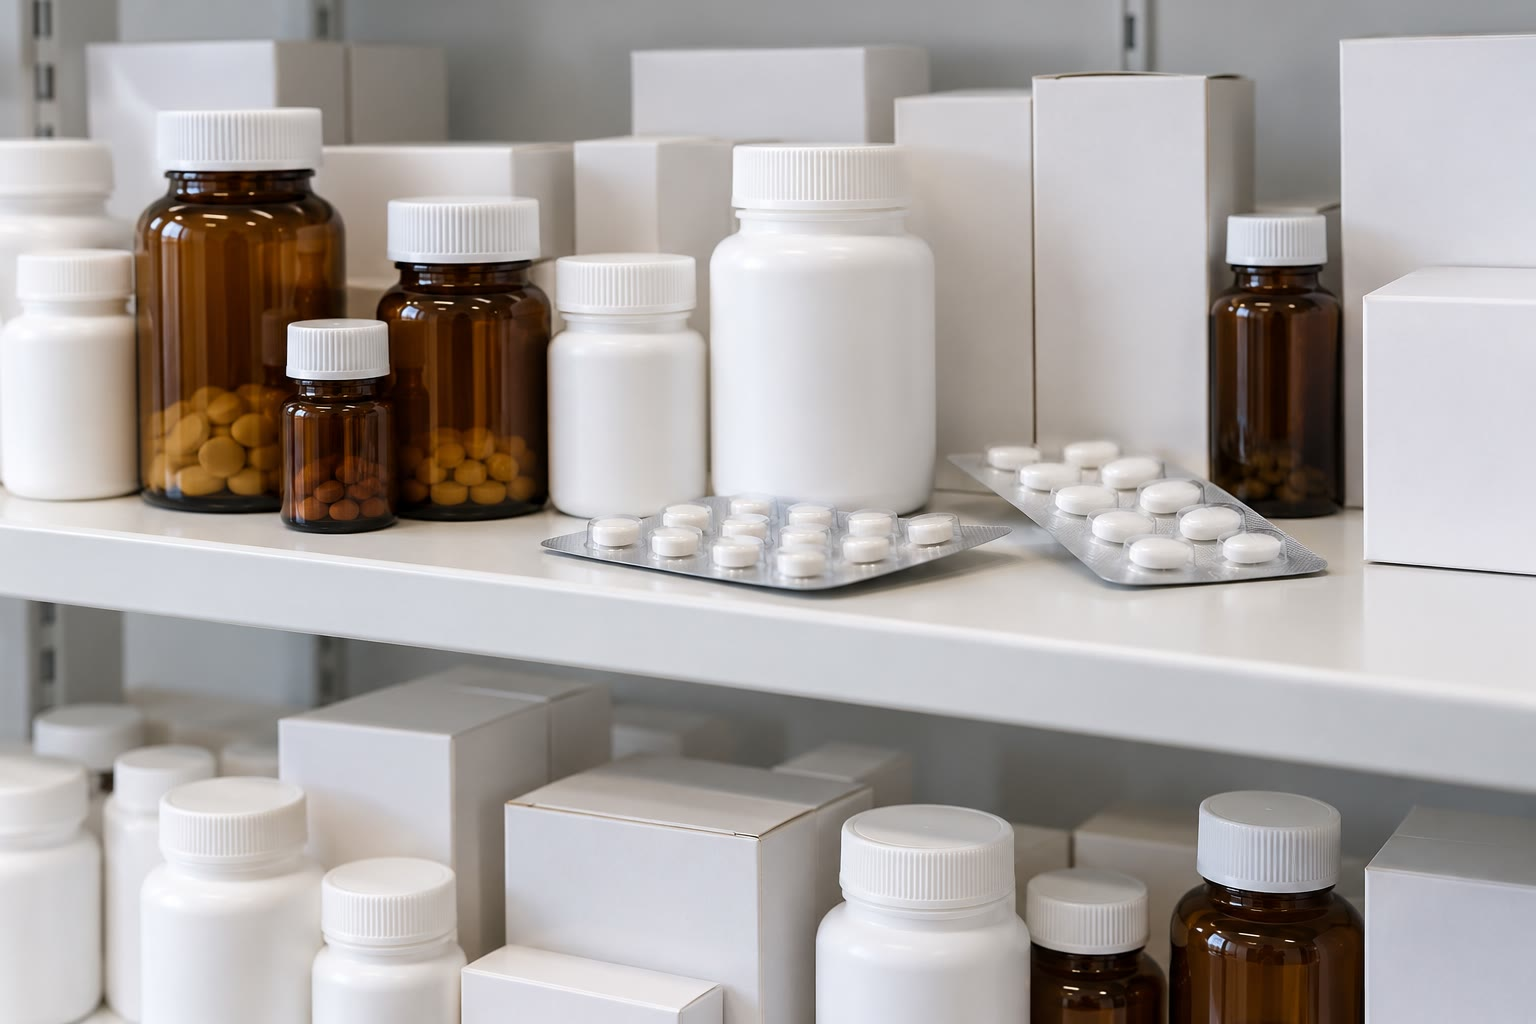
\includegraphics[width=0.6\linewidth]{images/book4/ai/b3-12-pharmacy.jpg}

{\small Medicines on a pharmacy shelf. Replacing hydrogen by deuterium at the
bonds the liver attacks first can lengthen the time a drug stays in the body.}
\end{omfigure}

\section{Collision theory}

Two molecules in a gas can react only if they meet. Model them as hard spheres
of diameters $d_{\mathrm A}$ and $d_{\mathrm B}$: they collide when their centres pass within $d =
\frac12(d_{\mathrm A} + d_{\mathrm B})$ of each other.

\begin{definition}[Collision cross-section, steric factor]\label{def:b3:rate-theories:collision}
The \emph{collision cross-section}\index{collision cross-section} of two molecules
is the area $\sigma = \pi d^2$ of the disc, perpendicular to their relative velocity,
inside which the centre of one must pass for it to hit the other. The
\emph{steric factor}\index{steric factor} $P$ is the ratio of the measured
pre-exponential factor of a reaction to the one predicted by collision theory.
\end{definition}

\begin{omfigure}
\begin{tikzpicture}[font=\small, >=Stealth]
  \shade[ball color=omDef!40] (0,0) circle (0.45);
  \node at (0,0) {A};
  \draw[black!50, dashed] (-0.0,0.85) -- (5.2,0.85) (-0.0,-0.85) -- (5.2,-0.85);
  \draw[black!60] (0,0) ellipse (0.25 and 0.85);
  \draw[<->] (-0.45,0) -- (-0.45,0.85) node[midway, left] {$d$};
  \shade[ball color=omThm!40] (3.3,0.55) circle (0.4);
  \node at (3.3,0.55) {B};
  \shade[ball color=omThm!20] (4.6,1.45) circle (0.4);
  \node at (4.6,1.45) {B};
  \draw[->, thick] (0.6,0) -- (2.2,0) node[midway, below] {$v_{\mathrm{rel}}\,\Delta t$};
  \node[anchor=west, align=left, font=\scriptsize] at (5.3,0) {cylinder of\\ cross-section\\ $\sigma = \pi d^2$};
  \node[font=\scriptsize, anchor=south] at (3.3,1.0) {hit};
  \node[font=\scriptsize, anchor=south] at (4.6,1.9) {missed};
\end{tikzpicture}

{\small The collision cylinder. Moving at the relative speed $v_{\mathrm{rel}}$, molecule A sweeps
in a time $\Delta t$ a cylinder of cross-section $\sigma = \pi d^2$, with $d$ the sum of the two
radii; every B whose centre lies inside is hit.}
\end{omfigure}

\begin{theorem}[Collision-theory rate constant]\label{thm:b3:rate-theories:collision}
If every collision whose kinetic energy along the line of centres exceeds a
threshold $E_0$ (per mole) leads to reaction, the rate constant of $\mathrm{A + B} \to$
products is
\[
  k = \sigma\bar v_{\mathrm{rel}}N_A\,\eu^{-E_0/RT}, \qquad \bar v_{\mathrm{rel}} = \sqrt{\frac{8kT}{\pi\mu}},\
  \mu = \frac{m_{\mathrm A}m_{\mathrm B}}{m_{\mathrm A} + m_{\mathrm B}} .
\]
\end{theorem}

\begin{proof}[Partial proof]
In a time $\Delta t$ a molecule A sweeps a volume $\sigma v_{\mathrm{rel}}\Delta t$ and hits the
$n_{\mathrm B}\sigma v_{\mathrm{rel}}\Delta t$ molecules B it contains: the collision rate per unit volume
is $\sigma\bar v_{\mathrm{rel}}n_{\mathrm A}n_{\mathrm B}$, with $\bar v_{\mathrm{rel}}$ the mean relative speed given by the
Maxwell--Boltzmann distribution (admitted from physics, with the \omterm{def:b3:quantum-model-systems:oscillator}{reduced
mass}). Weighting each collision by its speed and keeping those whose energy
along the line of centres exceeds the threshold leaves the fraction
$\eu^{-E_0/RT}$ of the collision rate (the integration over the impact parameter is
admitted). Converting number densities into molar concentrations multiplies by
$N_A$.
\end{proof}

Since $\bar v_{\mathrm{rel}} \propto \sqrt T$, the activation energy $E_a = RT^2\,\dd\ln k/\dd T$ is $E_0 + \frac12RT$,
close to the threshold. The pre-exponential factor is of the order of
$10^{11}$~\unit{L.mol^{-1}.s^{-1}} for small molecules. Measured factors are often
much smaller: $P \ll 1$ for molecules that must meet in a particular
orientation, and the cross-section has no unique value for real molecules,
which are not hard spheres. Collision theory gives the order of magnitude and
the temperature dependence; it cannot give $E_0$, which needs the \omterm{def:b3:computational-chemistry:pes}{potential
energy surface}.

\section{Potential energy surfaces}

The reaction $\mathrm{H_A + H_BH_C \to H_AH_B + H_C}$ is the simplest there is. For a collinear
approach the energy depends on two distances, $r_{\mathrm{AB}}$ and $r_{\mathrm{BC}}$, and can be drawn
as a map.

\begin{definition}[Saddle point, minimum energy path]\label{def:b3:rate-theories:saddle}
A \emph{saddle point}\index{saddle point} of a \omterm{def:b3:computational-chemistry:pes}{potential energy surface} is a point
where the gradient vanishes, the energy is a maximum along one direction and a
minimum along all others. The \emph{minimum energy path}\index{minimum energy
path} is the path of steepest descent from the saddle point to the reactant
and product valleys; its length measured along it is the reaction coordinate,
and the saddle point is the transition state.
\end{definition}

\begin{omfigure}
\begin{tikzpicture}
\begin{axis}[ompes, width=0.62\linewidth, xmin=0.4, xmax=3.0, ymin=0.4, ymax=3.0,
  xlabel={$r_{\mathrm{AB}}$ / \AA}, ylabel={$r_{\mathrm{BC}}$ / \AA},
  colorbar, colorbar style={ylabel={$E$ / eV}, ylabel style={font=\small},
  yticklabel style={font=\small}}, point meta min=-4.7, point meta max=-0.8]
\addplot3[contour prepared={labels=false}, thick] table {figdata/out/bachelor-3-pes-collinear-contours.dat};
\addplot3[ompath] table[x=x, y=y, z expr=0] {figdata/out/bachelor-3-pes-collinear-mep.dat};
\node[omsaddle] at (axis cs:0.918,0.918,0) {};
\node[font=\small, anchor=south west] at (axis cs:0.95,0.95,0) {saddle};
\node[font=\small, anchor=west, fill=white, fill opacity=0.85, text opacity=1, inner sep=1.5pt] at (axis cs:2.05,1.0,0) {$\mathrm{H_A + H_BH_C}$};
\node[font=\small, anchor=west, fill=white, fill opacity=0.85, text opacity=1, inner sep=1.5pt] at (axis cs:0.95,2.55,0) {$\mathrm{H_AH_B + H_C}$};
\node[font=\small, anchor=north east] at (axis cs:2.95,2.95,0) {$\ce{H + H + H}$};
\end{axis}
\end{tikzpicture}

{\small A model \omterm{def:b3:computational-chemistry:pes}{potential energy surface} for collinear $\ce{H + H2}$ (LEPS form built
from the Morse curve of \ce{H2}, with a Sato parameter of 0.17 chosen as a model
constant). Contours from \qty{-4.65}{eV} to \qty{-0.8}{eV}, energy zero for three separate atoms;
the valleys lie at \qty{-4.75}{eV}, the depth of the \ce{H2} well. Dashed: the \omterm{def:b3:rate-theories:saddle}{minimum
energy path}, which crosses the symmetric saddle at $r_{\mathrm{AB}} = r_{\mathrm{BC}} = \qty{0.92}{\AA}$,
\qty{0.27}{eV} above the valleys in this model.}
\end{omfigure}

The path climbs out of the reactant valley, where $r_{\mathrm{BC}}$ stays near the \ce{H2}
bond length while A approaches, crosses the saddle, and descends into the
product valley. At the saddle both bonds are stretched to \qty{0.92}{\AA}: the old
bond is half broken and the new one half made, and the energy cost of this
compromise is the barrier. For the symmetric reaction the saddle lies on the
diagonal; for an exothermic reaction it moves towards the reactant valley (an
early barrier, a reactant-like transition state, as the Hammond postulate
says), for an endothermic one towards the product valley (a late barrier).
The position decides which energy helps: translational energy, directed along
the entrance valley, carries the molecules over an early barrier; a late
barrier, around a corner, is crossed more easily with vibrational energy in the
breaking bond. These are Polanyi's rules, confirmed by molecular-beam
experiments.

\section{Transition-state theory}

\begin{definition}[Activated complex]\label{def:b3:rate-theories:activated-complex}
The \emph{activated complex}\index{activated complex} of an elementary step is the
set of configurations of the reacting system in a thin slice around the
\omterm{def:b3:rate-theories:saddle}{saddle point}, perpendicular to the \omterm{def:b3:rate-theories:saddle}{minimum energy path}; it is treated as a
species $\ce{AB^{\ddagger}}$, with its own partition function.
\end{definition}

\begin{definition}[Transition-state theory, transmission coefficient]\label{def:b3:rate-theories:tst}
\emph{Transition-state theory}\index{transition-state theory} assumes that the
\omterm{def:b3:rate-theories:activated-complex}{activated complexes} are in equilibrium with the reactants, that every complex
crossing the saddle region towards the products goes on to form them, and that
the motion along the reaction coordinate is a free translation. The
\emph{transmission coefficient}\index{transmission coefficient} $\kappa \le 1$ corrects for
the complexes that recross back to the reactants.
\end{definition}

\begin{theorem}[Eyring equation]\label{thm:b3:rate-theories:eyring}
For an elementary step $\mathrm{A + B} \to \mathrm{AB}^{\ddagger} \to$ products,
\[
  k = \kappa\frac{k_BT}{h}\overline{K}{}^{\ddagger}, \qquad
  \overline{K}{}^{\ddagger} = \frac{\bar q^{\ddagger}/N_A}{(q_{\mathrm A}/N_A)(q_{\mathrm B}/N_A)}\,\eu^{-\Delta E_0^{\ddagger}/RT},
\]
where $\bar q^{\ddagger}$ is the partition function of the \omterm{def:b3:rate-theories:activated-complex}{activated complex} with the
reaction-coordinate motion removed, $q$ are molar partition functions per unit
volume, and $\Delta E_0^{\ddagger}$ is the height of the zero-point level of the complex above
that of the reactants. In thermodynamic form, with $c^\circ = \qty{1}{mol/L}$ and the
molecularity $m$,
\[
  k = \kappa\frac{k_BT}{h}(c^\circ)^{1-m}\,\eu^{\Delta^{\ddagger}S^\circ/R}\,\eu^{-\Delta^{\ddagger}H^\circ/RT}.
\]
This statement is the \emph{Eyring equation}\index{Eyring equation}; $k_B$ is the
Boltzmann constant, written so to avoid confusion with $k$.
\end{theorem}

\begin{proof}
Quasi-equilibrium: $[\ce{AB^{\ddagger}}] = K^{\ddagger}[\mathrm A][\mathrm B]$, with $K^{\ddagger}$ from the partition functions
(\cref{thm:b3:statistical-thermo-applied:k-from-q}, written with concentrations).
Of the vibrations of the complex, one is the motion along the reaction
coordinate: a very loose vibration of frequency $\nu \ll k_BT/h$, whose partition
function is $k_BT/h\nu$ (the high-temperature limit of
\cref{prop:b3:partition-functions:q-vib}); hence $q^{\ddagger} = \bar q^{\ddagger}k_BT/h\nu$. The
complexes cross towards the products at the frequency $\nu$ of this motion, so the
rate is $\nu[\ce{AB^{\ddagger}}] = \nu\frac{k_BT}{h\nu}\overline{K}{}^{\ddagger}[\mathrm A][\mathrm B]$: the unknown $\nu$ cancels. Writing
$\overline{K}{}^{\ddagger} = (c^\circ)^{1-m}\eu^{-\Delta^{\ddagger}G^\circ/RT}$ and $\Delta^{\ddagger}G^\circ = \Delta^{\ddagger}H^\circ - T\Delta^{\ddagger}S^\circ$ gives the
second form, with $\kappa$ inserted for recrossing.
\end{proof}

The factor $k_BT/h$ is \qty{6.2e12}{s^{-1}} at \qty{298}{K}: the rate of a unimolecular step
with no barrier and no entropy loss. Everything specific to the reaction lies
in the quantities of activation.

\begin{definition}[Gibbs energy, enthalpy and entropy of activation]\label{def:b3:rate-theories:activation}
The \emph{Gibbs energy of activation}\index{Gibbs energy of activation}
$\Delta^{\ddagger}G^\circ$, \emph{enthalpy of activation}\index{enthalpy of activation} $\Delta^{\ddagger}H^\circ$ and
\emph{entropy of activation}\index{entropy of activation} $\Delta^{\ddagger}S^\circ$ of an elementary
step are the standard Gibbs energy, enthalpy and entropy of formation of the
\omterm{def:b3:rate-theories:activated-complex}{activated complex} (without its reaction-coordinate motion) from the reactants,
defined by the \omterm{thm:b3:rate-theories:eyring}{Eyring equation}.
\end{definition}

\begin{proposition}[Activation energy and enthalpy of activation]\label{prop:b3:rate-theories:ea-dh}
For a reaction in solution, $E_a = \Delta^{\ddagger}H^\circ + RT$; for a bimolecular gas reaction,
$E_a = \Delta^{\ddagger}H^\circ + 2RT$.
\end{proposition}

\begin{proof}
$E_a = RT^2\,\dd\ln k/\dd T$, and $\ln k = \ln T + \Delta^{\ddagger}S^\circ/R - \Delta^{\ddagger}H^\circ/RT + $ const: $E_a =
RT + \Delta^{\ddagger}H^\circ$ when the activation parameters do not vary with $T$. In solution
this is the result. In the gas phase the van 't Hoff relation for $K^{\ddagger}$ written
in concentrations involves the internal energy, $\Delta^{\ddagger}U^\circ = \Delta^{\ddagger}H^\circ - \Delta n^{\ddagger}RT$
with $\Delta n^{\ddagger} = 1 - m$: for $m = 2$, $E_a = \Delta^{\ddagger}H^\circ + 2RT$.
\end{proof}

The \omterm{def:b3:rate-theories:activation}{entropy of activation} reads the structure of the transition state. Two
molecules that combine into one complex lose translational and rotational
freedom: $\Delta^{\ddagger}S^\circ$ is strongly negative, $-50$ to $-150$ \unit{J.K^{-1}.mol^{-1}}, for
associative steps and cyclic transition states. A molecule that loosens a bond
on its way to dissociating gains freedom: $\Delta^{\ddagger}S^\circ > 0$.

\begin{proposition}[Standard errors of a fitted line]\label{prop:b3:rate-theories:slope-uncertainty}
For a least-squares line $y = a + bx$ through $n$ points whose $y$ carry
independent errors of the same variance, estimated by $s^2 = \sum_i(y_i - a - bx_i)^2/(n - 2)$,
the slope and intercept have the standard errors
\[
  s_b = \frac{s}{\sqrt{\sum_i(x_i - \bar x)^2}}, \qquad
  s_a = s\sqrt{\frac1n + \frac{\bar x^2}{\sum_i(x_i - \bar x)^2}} .
\]
\end{proposition}

\begin{proof}
$b = \sum_i(x_i - \bar x)y_i/S_{xx}$, with $S_{xx} = \sum_i(x_i - \bar x)^2$, is a linear combination of
independent $y_i$ of variance $\sigma^2$: its variance is $\sigma^2\sum_i(x_i - \bar x)^2/S_{xx}^2 = \sigma^2/S_{xx}$.
Likewise $a = \bar y - b\bar x$, and $\bar y$ and $b$ are uncorrelated (their covariance is
$\sigma^2\sum_i(x_i - \bar x)/(nS_{xx}) = 0$), so $\operatorname{var}a = \sigma^2/n + \bar x^2\sigma^2/S_{xx}$. Replacing $\sigma^2$
by its estimate $s^2$ (the divisor $n - 2$ accounts for the two fitted
parameters, admitted) gives the result.
\end{proof}

\begin{method}[An Eyring plot with uncertainties]\label{met:b3:rate-theories:eyring-plot}
\begin{enumerate}
  \item Measure $k$ at five or more temperatures spread over 30 to \qty{40}{K}.
  \item Plot $y = \ln(k/T)$ against $x = 1/T$ and fit the least-squares line $y = a + bx$.
  \item $\Delta^{\ddagger}H^\circ = -Rb$ and $\Delta^{\ddagger}S^\circ = R[a - \ln(k_B/h)]$ ($\ln(k_B/h) = 23.760$ with $k$ in
        \unit{s^{-1}}).
  \item Their standard errors are $Rs_b$ and $Rs_a$; a 95\,\% confidence interval
        multiplies them by Student's $t$ for $n - 2$ degrees of freedom (3.18 for
        five points).
  \item The intercept lies far outside the measured range, at $1/T = 0$: $\Delta^{\ddagger}S^\circ$
        is always much less precise than $\Delta^{\ddagger}H^\circ$, and the two errors are
        correlated.
\end{enumerate}
\end{method}

\begin{omfigure}
\begin{tikzpicture}
\begin{axis}[width=0.74\linewidth, height=6.2cm, xmin=3.12, xmax=3.62, ymin=-12.8, ymax=-6.4,
  axis lines=left, xlabel={$1000\,\mathrm K/T$}, ylabel={$\ln\bigl(k/(\mathrm s^{-1}\,\mathrm K^{-1})\bigr)$},
  tick label style={font=\small}, label style={font=\small},
  legend style={font=\scriptsize, draw=none, fill=white, fill opacity=0.85, text opacity=1,
  at={(0.98,0.98)}, anchor=north east}, legend cell align=left]
\addplot[omDef, thick] table[x=invT, y=fit] {figdata/out/bachelor-3-eyring-band-H.dat};
\addplot[omThm, thick] table[x=invT, y=fit] {figdata/out/bachelor-3-eyring-band-D.dat};
\addplot[omDef, thin, dashed, forget plot] table[x=invT, y=lo] {figdata/out/bachelor-3-eyring-band-H.dat};
\addplot[omDef, thin, dashed, forget plot] table[x=invT, y=hi] {figdata/out/bachelor-3-eyring-band-H.dat};
\addplot[omThm, thin, dashed, forget plot] table[x=invT, y=lo] {figdata/out/bachelor-3-eyring-band-D.dat};
\addplot[omThm, thin, dashed, forget plot] table[x=invT, y=hi] {figdata/out/bachelor-3-eyring-band-D.dat};
\addplot[only marks, mark=*, mark size=1.8pt, omDef, forget plot] table[x=invT, y=lnkT_H] {figdata/out/bachelor-3-eyring-points.dat};
\addplot[only marks, mark=square*, mark size=1.7pt, omThm, forget plot] table[x=invT, y=lnkT_D] {figdata/out/bachelor-3-eyring-points.dat};
\legend{\ce{OCH3} drug, \ce{OCD3} drug}
\end{axis}
\end{tikzpicture}

{\small Eyring plots of the weekend problem's rate constants (data of the
problem) for the drug and its deuterated analogue, with the least-squares lines
and their 95\,\% confidence bands (dashed, hardly wider than the lines: the
points scatter by about 1\,\%). The lines are parallel within their
uncertainty: the same \omterm{def:b3:rate-theories:activation}{entropy of activation}, enthalpies of activation that
differ by about \qty{5}{kJ/mol}.}
\end{omfigure}

\section{Kinetic isotope effects}

\begin{definition}[Kinetic isotope effects]\label{def:b3:rate-theories:kie}
The \emph{kinetic isotope effect}\index{kinetic isotope effect} of a step is the
ratio $k_{\mathrm{light}}/k_{\mathrm{heavy}}$ of its rate constants for two \omterm{def:b3:rovibrational-spectroscopy:rotational-constant}{isotopologues}, most often
$k_{\mathrm H}/k_{\mathrm D}$. It is a \emph{primary kinetic isotope effect}\index{primary kinetic
isotope effect} when the bond to the substituted atom is made or broken in the
step, a \emph{secondary kinetic isotope effect}\index{secondary kinetic isotope
effect} when it is not.
\end{definition}

\begin{proposition}[Maximum primary kinetic isotope effect]\label{prop:b3:rate-theories:primary-kie}
If the stretching vibration of an X--H bond becomes the reaction coordinate,
so that its \omterm{def:b3:quantum-model-systems:oscillator}{zero-point energy} is lost in the transition state while all other
contributions are the same for H and D,
\[
  \frac{k_{\mathrm H}}{k_{\mathrm D}} = \exp\Bigl[\frac{hc(\tilde\nu_{\mathrm{XH}} - \tilde\nu_{\mathrm{XD}})}{2k_BT}\Bigr],
  \qquad \frac{\tilde\nu_{\mathrm{XH}}}{\tilde\nu_{\mathrm{XD}}} = \sqrt{\frac{\mu_{\mathrm{XD}}}{\mu_{\mathrm{XH}}}} .
\]
\end{proposition}

\begin{proof}
The \omterm{def:b3:computational-chemistry:pes}{potential energy surface} is the same for both \omterm{def:b3:rovibrational-spectroscopy:rotational-constant}{isotopologues} (the
electrons do not see the neutron). In the reactant the X--H stretch holds
$\frac12hc\tilde\nu_{\mathrm{XH}}$ of \omterm{def:b3:quantum-model-systems:oscillator}{zero-point energy}; in the transition state this mode has become
the reaction coordinate and holds none. The barrier measured between zero-point
levels is therefore lower for H by $\frac12hc\tilde\nu_{\mathrm{XH}}$ and for D by $\frac12hc\tilde\nu_{\mathrm{XD}}$: $\Delta E_0^{\ddagger}(\mathrm D) -
\Delta E_0^{\ddagger}(\mathrm H) = \frac12hc(\tilde\nu_{\mathrm{XH}} - \tilde\nu_{\mathrm{XD}})$, and the \omterm{thm:b3:rate-theories:eyring}{Eyring equation} gives the ratio when
the other factors cancel. The wavenumber of a stretch is proportional to
$1/\sqrt\mu$ (\cref{ch:b3:rovibrational-spectroscopy}).
\end{proof}

\begin{omfigure}
\begin{tikzpicture}[font=\small, >=Stealth, x=1cm, y=1cm]
  \draw[->] (-1.4,0) -- (-1.4,4.7) node[anchor=south] {$E$};
  \draw[->] (-1.4,0) -- (10.6,0) node[anchor=north east] {reaction coordinate};
  \draw[very thick, black!70] plot[smooth, tension=0.6] coordinates {(1.6,3.4) (2.1,1.6) (2.7,0.8)
    (3.3,0.6) (3.9,0.8) (4.7,2.0) (5.5,3.6) (6.2,4.0) (6.9,3.6) (7.7,2.2) (8.5,1.2) (9.2,1.0)
    (9.9,1.2) (10.4,1.7)};
  \draw[black!50, dashed] (2.8,0.6) -- (3.8,0.6);
  \draw[omDef, thick] (2.42,1.35) -- (4.2,1.35);
  \draw[omThm, thick] (2.5,1.05) -- (4.05,1.05);
  \node[omDef, font=\scriptsize, anchor=south] at (3.3,1.37) {C--H};
  \node[omThm, font=\scriptsize, anchor=north] at (3.3,1.03) {C--D};
  \draw[black, thick] (5.7,4.0) -- (6.7,4.0);
  \draw[black!40, densely dotted] (0.0,4.0) -- (5.7,4.0);
  \draw[black!40, densely dotted] (0.7,1.35) -- (2.42,1.35) (0.0,1.05) -- (2.5,1.05);
  \draw[<->, omThm] (0.0,1.05) -- (0.0,4.0) node[pos=0.5, left, font=\scriptsize] {$E_0(\mathrm D)$};
  \draw[<->, omDef] (0.7,1.35) -- (0.7,4.0) node[pos=0.5, right, font=\scriptsize] {$E_0(\mathrm H)$};
  \node[anchor=south, align=center, font=\scriptsize] at (6.2,4.05) {transition state: the stretch has\\ become the reaction coordinate};
\end{tikzpicture}

{\small Origin of the \omterm{def:b3:rate-theories:kie}{primary kinetic isotope effect}. In the reactant, the C--H
stretch holds more \omterm{def:b3:quantum-model-systems:oscillator}{zero-point energy} than the C--D stretch (levels above the
bottom of the well, dashed); in the transition state this vibration has become
the reaction coordinate, and both \omterm{def:b3:rovibrational-spectroscopy:rotational-constant}{isotopologues} reach the same top. The
barrier is larger for D by the difference of the zero-point energies.}
\end{omfigure}

\begin{omfigure}
\begin{tikzpicture}
\begin{axis}[width=0.7\linewidth, height=5.6cm, xmin=200, xmax=800, ymin=1, ymax=50,
  ymode=log, axis lines=left, xlabel={$T$ / K}, ylabel={$k_{\mathrm H}/k_{\mathrm D}$ (maximum)},
  tick label style={font=\small}, label style={font=\small}, log ticks with fixed point,
  ytick={1,2,5,10,20,50}, legend style={font=\scriptsize, draw=none, at={(0.98,0.98)},
  anchor=north east}, legend cell align=left]
\addplot[omThm, thick] table[x=T, y=OH] {figdata/out/bachelor-3-kie.dat};
\addplot[black!60, thick] table[x=T, y=NH] {figdata/out/bachelor-3-kie.dat};
\addplot[omDef, thick] table[x=T, y=CH] {figdata/out/bachelor-3-kie.dat};
\legend{O--H (\qty{3657}{cm^{-1}}), N--H (\qty{3337}{cm^{-1}}), C--H (\qty{2917}{cm^{-1}})}
\end{axis}
\end{tikzpicture}

{\small Maximum \omterm{def:b3:rate-theories:kie}{primary kinetic isotope effect} against temperature for the loss
of a C--H, N--H or O--H stretch (fundamentals of \ce{CH4}, \ce{NH3} and \ce{H2O}; the
deuterium wavenumbers from the reduced masses). At \qty{298}{K} it is 6.5 for C--H;
it decreases towards 1 as the temperature rises.}
\end{omfigure}

The maximum C--H value at room temperature, about 7, is a benchmark. Observed
effects of 2 to 7 indicate that the C--H bond is broken in the rate-determining
step; smaller values that the transition state keeps part of the stretch
(asymmetric, early or late hydrogen transfers), or that the step is not the
slowest. Values much larger than 7 at room temperature cannot come from
zero-point energies: they reveal \omterm{def:b3:quantum-model-systems:tunnelling}{tunnelling} (\cref{ch:b3:quantum-model-systems}),
which a particle of twice the mass does much less. Secondary effects, from
changes of the bending vibrations of C--H bonds next to the reacting centre,
are small, typically 0.8 to 1.2 per deuterium; they distinguish, for example, a
carbon that becomes trigonal (sp³ to sp², $k_{\mathrm H}/k_{\mathrm D} > 1$) from one that becomes
tetrahedral ($< 1$).

\begin{method}[Measuring a kinetic isotope effect by competition]\label{met:b3:rate-theories:kie}
\begin{enumerate}
  \item Run the reaction on a mixture of the two \omterm{def:b3:rovibrational-spectroscopy:rotational-constant}{isotopologues}, or on a
        molecule carrying H on one site and D on an equivalent one.
  \item Stop at low conversion and measure the ratio of the H and D products by
        mass spectrometry or NMR.
  \item The product ratio, corrected for the starting ratio, is $k_{\mathrm H}/k_{\mathrm D}$; both
        \omterm{def:b3:rovibrational-spectroscopy:rotational-constant}{isotopologues} see exactly the same conditions, which makes the method
        more precise than two separate rate measurements.
\end{enumerate}
\end{method}

\section{Reactions in solution}

In a liquid a molecule does not fly freely between collisions: it rattles in a
cage of neighbours, colliding with them many times before it diffuses away.
Two reactants that meet stay together for many collisions, an encounter.

\begin{definition}[Diffusion and activation control, cage effect]\label{def:b3:rate-theories:diffusion}
A reaction in solution is \emph{diffusion-controlled}\index{diffusion-controlled
reaction} when reaction at every encounter is fast, so that its rate is the rate
at which the reactants diffuse together; it is
\emph{activation-controlled}\index{activation-controlled reaction} when only a small
fraction of encounters lead to reaction. The \emph{cage effect}\index{cage
effect} is the confinement of a pair of molecules by the surrounding solvent,
which makes them collide repeatedly during one encounter.
\end{definition}

\begin{proposition}[Smoluchowski limit]\label{prop:b3:rate-theories:smoluchowski}
The rate constant of a \omterm{def:b3:rate-theories:diffusion}{diffusion-controlled reaction} between spheres that react
at the distance $R^*$ is $k_d = 4\pi N_A(D_{\mathrm A} + D_{\mathrm B})R^*$. With the Stokes--Einstein
relation $D = k_BT/6\pi\eta a$ for spheres of radius $a$ in a solvent of viscosity $\eta$,
and $R^* = a_{\mathrm A} + a_{\mathrm B}$ with $a_{\mathrm A} = a_{\mathrm B}$,
\[
  k_d = \frac{8RT}{3\eta} .
\]
\end{proposition}

\begin{proof}[Partial proof]
Fix A at the origin; B diffuses with the relative diffusion coefficient $D =
D_{\mathrm A} + D_{\mathrm B}$ and is destroyed at $r = R^*$. In the steady state the radial flux
through every sphere is the same, $J = 4\pi r^2D\,\dd c/\dd r$ (Fick's law, from
physics); integrating from $R^*$, where $c = 0$, to infinity, where $c = c_{\mathrm B}$, gives
$J = 4\pi DR^*c_{\mathrm B}$, the rate per molecule A. With Stokes--Einstein (admitted),
$(D_{\mathrm A} + D_{\mathrm B})R^* = \frac{k_BT}{6\pi\eta}(\frac{1}{a} + \frac1a)(2a) = \frac{2k_BT}{3\pi\eta}$, and $k_d = 4\pi N_A \times
\frac{2k_BT}{3\pi\eta} = 8RT/3\eta$.
\end{proof}

\begin{example}[Speed limits in water and in hexane]\label{ex:b3:rate-theories:speed-limit}
% ledger: visc:H2O.25C, visc:hexane.25C
At \qty{298.15}{K}, water ($\eta = \qty{0.890}{mPa.s}$) gives $k_d = 8 \times 8.314 \times
298.15/(3 \times \num{0.890e-3}) = \qty{7.4e6}{m^3.mol^{-1}.s^{-1}} = \qty{7.4e9}{L.mol^{-1}.s^{-1}}$; hexane
($\eta = \qty{0.298}{mPa.s}$), \qty{2.2e10}{L.mol^{-1}.s^{-1}}. No bimolecular reaction between
neutral molecules of ordinary size is faster; measured constants near these
values (the quenching of excited states, the recombination of radicals) are
\omterm{def:b3:rate-theories:diffusion}{diffusion-controlled}. Ions of opposite charge attract and can go faster.
\end{example}

Ions in solution add an electrostatic contribution to the activation: the
transition state of two ions has charge $z_{\mathrm A} + z_{\mathrm B}$, and its activity coefficient
differs from the product of theirs.

\begin{definition}[Kinetic salt effect]\label{def:b3:rate-theories:salt}
The \emph{kinetic salt effect}\index{kinetic salt effect} is the change of the rate
constant of a reaction between ions with the ionic strength of the solution.
\end{definition}

\begin{proposition}[Brønsted--Bjerrum equation]\label{prop:b3:rate-theories:bronsted-bjerrum}
For a step between ions of charges $z_{\mathrm A}$ and $z_{\mathrm B}$ in dilute aqueous solution,
\[
  \log k = \log k_0 + 2Az_{\mathrm A}z_{\mathrm B}\sqrt I,
\]
where $k_0$ is the rate constant at zero ionic strength.
\end{proposition}

\begin{proof}
In \omterm{def:b3:rate-theories:tst}{transition-state theory} the equilibrium with the \omterm{def:b3:rate-theories:activated-complex}{activated complex} is written
with activities: $[\ce{AB^{\ddagger}}] = K^{\ddagger}[\mathrm A][\mathrm B]\gamma_{\mathrm A}\gamma_{\mathrm B}/\gamma^{\ddagger}$, so $k = k_0\gamma_{\mathrm A}\gamma_{\mathrm B}/\gamma^{\ddagger}$.
With the limiting law: $\log(\gamma_{\mathrm A}\gamma_{\mathrm B}/\gamma^{\ddagger}) = -A\sqrt I[z_{\mathrm A}^2 + z_{\mathrm B}^2 - (z_{\mathrm A} + z_{\mathrm B})^2] =
2Az_{\mathrm A}z_{\mathrm B}\sqrt I$.
\end{proof}

Ions of the same sign react faster when salt is added (the ionic atmosphere
screens their repulsion), ions of opposite signs more slowly, and a neutral
reactant shows no primary salt effect: a plot of $\log k$ against $\sqrt I$ at low
ionic strength measures the product of the charges of the reacting species.

\begin{method}[What activation parameters say about a mechanism]\label{met:b3:rate-theories:mechanism-evidence}
\begin{enumerate}
  \item $\Delta^{\ddagger}S^\circ$ strongly negative: an associative step, an ordered or cyclic
        transition state, or one that orders the solvent (charge creation);
        positive: a dissociative step.
  \item A primary $k_{\mathrm H}/k_{\mathrm D}$ of 2 to 7: the bond to H is broken in the
        rate-determining step; above about 10 at room temperature: \omterm{def:b3:quantum-model-systems:tunnelling}{tunnelling}.
  \item The slope of $\log k$ against $\sqrt I$: the product $z_{\mathrm A}z_{\mathrm B}$ of the charges that
        meet in the rate-determining step.
  \item A rate constant near $10^{10}$~\unit{L.mol^{-1}.s^{-1}} that varies as $T/\eta$:
        diffusion control.
\end{enumerate}
\end{method}

\begin{inthelab}[A jacketed cell for an Eyring study]
The reaction is followed by its absorbance in a spectrophotometer cell whose
jacket is fed by a thermostated bath; a thermocouple in a reference cell checks
the temperature to \qty{0.1}{K}. Five to seven temperatures, each measured in
triplicate, give an Eyring plot; the solutions are equilibrated in the
holder before mixing, since a reaction started at the wrong temperature biases
the first points.
\end{inthelab}

\begin{history}[Eyring, Evans and Polanyi, 1935]
In 1935 Henry Eyring, in Princeton, and Meredith Gwynne Evans and Michael
Polanyi, in Manchester, published independently the theory of the \omterm{def:b3:rate-theories:activated-complex}{activated
complex}. Eyring had computed, with Polanyi in Berlin in 1931, the first
\omterm{def:b3:computational-chemistry:pes}{potential energy surface} for $\ce{H + H2}$, by a semi-empirical method of the kind used
for the figure of this chapter. The theory was received with suspicion: a
journal first rejected Eyring's paper as unsound, and it was published only
after other physicists vouched for it.
\end{history}

\section{Exercises}

\begin{exercise}[$\star$]\label{exo:b3:rate-theories:1}
% ledger: kin:NO+O3.A
For $\ce{NO + O3 -> NO2 + O2}$ take $\sigma = \qty{0.43}{nm^2}$ (data of the exercise). Compute $\bar v_{\mathrm{rel}}$
at \qty{298}{K} ($\mu = \qty{18.46}{u}$), the collision-theory pre-exponential factor, and the
\omterm{def:b3:rate-theories:collision}{steric factor} given the measured $A = \qty{2.07e-12}{cm^3.molecule^{-1}.s^{-1}}$.
\end{exercise}

\begin{exercise}[$\star$]\label{exo:b3:rate-theories:2}
A reaction in solution has $E_a = \qty{75.0}{kJ/mol}$ near \qty{298}{K}. What is $\Delta^{\ddagger}H^\circ$? And
for a bimolecular gas reaction with the same $E_a$?
\end{exercise}

\begin{exercise}[$\star$]\label{exo:b3:rate-theories:3}
Predict the sign of $\Delta^{\ddagger}S^\circ$ for: a Diels--Alder cycloaddition; the
unimolecular loss of \ce{N2} from an azo compound; an $\mathrm{S_N2}$ reaction between two
neutral molecules that creates two ions in a polar solvent.
\end{exercise}

\begin{exercise}[$\star$]\label{exo:b3:rate-theories:4}
% ledger: visc:H2O.25C, visc:hexane.25C
Compute the \omterm{def:b3:rate-theories:diffusion}{diffusion-controlled} rate constant in water and in hexane at
\qty{298.15}{K}. Which solvent allows faster encounters, and why?
\end{exercise}

\begin{exercise}[$\star\star$]\label{exo:b3:rate-theories:5}
A first-order reaction has $k = \qty{1.00e-3}{s^{-1}}$ at \qty{298.15}{K} and \qty{1.00e-2}{s^{-1}} at
\qty{318.15}{K}. Compute $\Delta^{\ddagger}H^\circ$ and $\Delta^{\ddagger}S^\circ$, and $E_a$ for comparison.
\end{exercise}

\begin{exercise}[$\star\star$]\label{exo:b3:rate-theories:6}
% ledger: vib:H2O.sym
Compute the maximum primary isotope effect for the transfer of an O--H proton at
\qty{298}{K} ($\tilde\nu_{\mathrm{OH}} = \qty{3657}{cm^{-1}}$, reduced masses with O = 16, H = 1, D = 2).
\end{exercise}

\begin{exercise}[$\star\star$]\label{exo:b3:rate-theories:7}
% ledger: vib:CH4.nu1, vib:CD4.nu1
An enzymatic hydrogen transfer from carbon shows $k_{\mathrm H}/k_{\mathrm D} = 40$ at \qty{298}{K}. Compare
with the maximum from zero-point energies ($\tilde\nu = 2917$ and \qty{2109}{cm^{-1}}) and conclude.
\end{exercise}

\begin{exercise}[$\star\star$]\label{exo:b3:rate-theories:8}
Predict the effect of raising the ionic strength from 0 to 0.010 on the rate
of: the oxidation of \ce{I-} by \ce{S2O8^{2-}} (rate-determining step between these two ions); the
reaction of \ce{CH3COOC2H5} with \ce{OH-}; the reaction of $\ce{[Co(NH3)5Br]^{2+}}$ with \ce{OH-}.
Give the factor where there is one ($A = 0.51$).
\end{exercise}

\begin{exercise}[$\star\star$]\label{exo:b3:rate-theories:9}
The reaction $\ce{F + H2 -> HF + H}$ is strongly exothermic. Where is its barrier on the
\omterm{def:b3:computational-chemistry:pes}{potential energy surface}? For the reverse reaction, which form of energy, given
to the reactants, best promotes it?
\end{exercise}

\begin{exercise}[$\star\star\star$]\label{exo:b3:rate-theories:10}
A least-squares fit of $\ln(k/T)$ against $1/T$ over five points gives $b = -7446$ K
with $s_b = \qty{31}{K}$ and $a = 16.528$ with $s_a = 0.103$. Give $\Delta^{\ddagger}H^\circ$ and $\Delta^{\ddagger}S^\circ$ with
their standard errors and 95\,\% confidence intervals ($t = 3.18$).
\end{exercise}

\begin{exercise}[$\star\star\star$]\label{exo:b3:rate-theories:11}
Starting from the \omterm{thm:b3:rate-theories:eyring}{Eyring equation}, show that $E_a = \Delta^{\ddagger}H^\circ + RT$ for a
unimolecular step and that $A = \eu\,(k_BT/h)\eu^{\Delta^{\ddagger}S^\circ/R}$. Deduce $A$ for $\Delta^{\ddagger}S^\circ = 0$ at
\qty{298}{K}, and compare with the $10^{13}$ to $10^{14}$~\unit{s^{-1}} of simple bond fissions.
\end{exercise}

\begin{exercise}[$\star\star\star$]\label{exo:b3:rate-theories:12}
Apply \omterm{def:b3:rate-theories:tst}{transition-state theory} to two structureless atoms A and B whose \omterm{def:b3:rate-theories:activated-complex}{activated
complex} is a diatomic of bond length $d$ (no vibration left once the reaction
coordinate is removed, rotation with $I = \mu d^2$). Show that it gives the
collision-theory rate constant with $\sigma = \pi d^2$.
\end{exercise}

\section{Problem: A Heavier Medicine}

\begin{problem}[{Weekend problem --- a heavier medicine: zero-point energies
of C--H and C--D stretches, the maximum isotope effect at body temperature, the
half-life of a deuterated drug, and an Eyring analysis of both compounds}]
\label{pb:b3:rate-theories:1}
% ledger: vib:CH4.nu1, vib:CD4.nu1, imass:H1, imass:H2, hist4:deut.2017
A drug is cleared from the body by two routes: 75\,\% of its clearance by the
O-demethylation of its two \ce{OCH3} groups, in which the cleavage of a C--H bond is
rate-determining, and 25\,\% by routes that do not touch these bonds; its
half-life is \qty{5.0}{h} (data of the problem). Its analogue carries two \ce{OCD3}
groups. Model C--H and C--D stretches: the symmetric stretches of \ce{CH4}
(\qty{2917}{cm^{-1}}) and \ce{CD4} (\qty{2109}{cm^{-1}}). First-order rate constants of the
demethylation step measured with a liver-enzyme preparation (data of the
problem):
\begin{center}\small
\begin{tabular}{lccccc}
\hline
$T$ / K & 278.15 & 288.15 & 298.15 & 308.15 & 318.15 \\
$k_{\mathrm H}$ / \unit{s^{-1}} & 0.00989 & 0.0263 & 0.0632 & 0.150 & 0.328 \\
$k_{\mathrm D}$ / \unit{s^{-1}} & 0.00117 & 0.00333 & 0.00874 & 0.0219 & 0.0503 \\ \hline
\end{tabular}
\end{center}

\medskip\noindent\textbf{Part I --- Zero-point energies.}
\begin{enumerate}
  \item Compute the reduced masses of C--H and C--D (C = 12, H = 1.00783,
        D = 2.01410).
  \item Predict the C--D wavenumber from the C--H one and compare with the
        measured \qty{2109}{cm^{-1}}.
  \item Compute the zero-point energies of the two stretches and their
        difference, in \unit{cm^{-1}} and \unit{kJ/mol} (measured wavenumbers).
  \item What happens to the stretching vibration of the bond being broken in
        the transition state?
  \item Deduce the difference of the barriers for H and D.
\end{enumerate}

\medskip\noindent\textbf{Part II --- The isotope effect.}
\begin{enumerate}[resume]
  \item Compute the maximum $k_{\mathrm H}/k_{\mathrm D}$ at \qty{37}{\celsius}.
  \item Compute it at \qty{25}{\celsius}.
  \item Why is it called a maximum?
  \item Do the two other deuterium atoms of each \ce{CD3} group contribute much?
  \item What does a measured value near 7 at \qty{25}{\celsius} say about the
        mechanism?
\end{enumerate}

\medskip\noindent\textbf{Part III --- Half-lives.}
\begin{enumerate}[resume]
  \item How does the half-life depend on the total clearance rate constant?
  \item Write the total rate constant of the H drug as the sum of its two
        routes, in fractions.
  \item By how much is the demethylation route slowed in the D drug?
  \item Compute $k_{\mathrm{total}}(\mathrm D)/k_{\mathrm{total}}(\mathrm H)$.
  \item Compute the half-life of the D drug.
  \item Compute the ratio of the half-lives.
  \item What would it be if the whole clearance went through demethylation?
  \item What does a longer half-life change for the patient?
\end{enumerate}

\medskip\noindent\textbf{Part IV --- An Eyring analysis.}
\begin{enumerate}[resume]
  \item Which plot of the data is linear according to the \omterm{thm:b3:rate-theories:eyring}{Eyring equation}?
  \item Fit it for the H drug: $\Delta^{\ddagger}H^\circ$ and $\Delta^{\ddagger}S^\circ$ with their standard errors.
  \item Do the same for the D drug.
  \item Compute $\Delta\Delta^{\ddagger}H^\circ = \Delta^{\ddagger}H^\circ(\mathrm D) - \Delta^{\ddagger}H^\circ(\mathrm H)$ and its standard error.
  \item Is it equal to the \omterm{def:b3:quantum-model-systems:oscillator}{zero-point energy} difference of question 3?
  \item What do the two entropies of activation say?
  \item State the result: the predicted ratio of the half-lives of the two drugs
        at \qty{37}{\celsius}.
\end{enumerate}
\end{problem}
